\section{Looking for Underlying Structure}
\label{sec:PCA}
The size of our testing set is 8965 $\times$ 342. However, we suspect that at least some of these data points are redundant. This section will explore some of the underlying structure of the data by looking at correlations between variables and employing dimension reduction techniques such as principal component analysis (PCA) and independent component analysis (ICA). 
\subsection{Correlations}
The first line of attack is to calculate the correlation matrix. It will provide two pieces of information. First, presence of large non-zero off-diagonal values in this matrix will be a good indication that redundant dimensions are present. Second, correlations of our response variable C1 with other variables might indicate which variables are tied most closely together with binge drinking. We applied cor() to the data, and sorted the results by column C1, which we earlier picked as the response variable. The top twenty variables are given in Table \ref{correlations}. These results are disappointing in the sense that we did not learn anything new about the data, merely discovered a lot of redundancy. Redundancy in the data can be addressed by applying dimension reduction using principal component analysis.

\begin{center}
\begin{table*}[ht]
\centering
\begin{tabular}{l l l}
\hline \hline
Correlation with C1 & Variable Name &Short summary of the variable given in the Codebook\\ \hline 
0.598 & D4A	&Compare own drinking to students\\
0.511 & G11	&High school-5 or more drinks in a row\\
-0.497 & A8F	&How important are parties\\
0.483 & D3A	&Max drinks male\\
0.472 & E27C	&Ride with high or drunk driver in past 30 days\\
0.460 & G10	&High school - drink per time\\
0.459 & E27E	&Ride with designated driver in past 30 days\\
0.454 & E1A	&Marijuana\\
0.451 & G9	&High school-drink per month\\
0.441 & D4B	&Compare own drinking to friends\\
\hline
\end{tabular}
\caption{Top 10 correlations with C1. Evidently, drinking is related to drinking. These data suggest that dimension reduction could be useful to get rid of redundant data and make the important relationships between alcohol and other variables clearer.}
\label{correlations}
\end{table*}
\end{center}

\subsection{Principal Component Analysis using Singular Value Decomposition}
A brief summary of singular value decomposition (SVD) follows \cite{berrar}. For a matrix $X$, we define left- and right-singular vectors, $u$ and $v$, such that:
\begin{equation}
Xv=su,~X^*u = sv;
\end{equation}
where each $s$ is a singular value of $X$. We are interested in finding these vectors because it can be shown that a least-squares approximation to $X$ equals $\sum_{k=1}^{l}u_ks_kv_k^T$. In order to take advantage of this property to analyze a $m\times n$ matrix $X$ containing $m$ observations of $n$ variables, we look to solve $X = USV^T$. Here $U$ contains a set of left singular vectors $u_k$, and $V$ contains the set of right singular vectors $v_k$, and $S$ is a diagonal matrix containing singular values $s_k$, where $k = 1, ..., n$. Solving $X = USV^T$ is equivalent to finding eigenvalue decompositions of $X^*X$ and $XX^*$, which can be performed analytically. 

In this subsection, we are using the standard R function prcomp(), which performs PCA using SVD, to reduce the number of variables to a handful of principal components. The first decision we need to make is the number of principal components we want to keep. Keeping fewer components means less work in performing regression, but at the risk of losing prediction accuracy. Keeping more components takes us closer to fitting the entire data set. It is helpful to plot the variance along each component, and stop increasing the number of components once the variance starts to drop off sharply. This plot is shown in Fig. \ref{components}. Unfortunately, no sharp drop-off is evident. In this section, we picked the number of components to equal four, because beginning with component three, the top variables start to get repeated from component to component. It will also be interesting to see how well four numbers can represent the data from ~200 variables. 
\begin{figure}
\centering
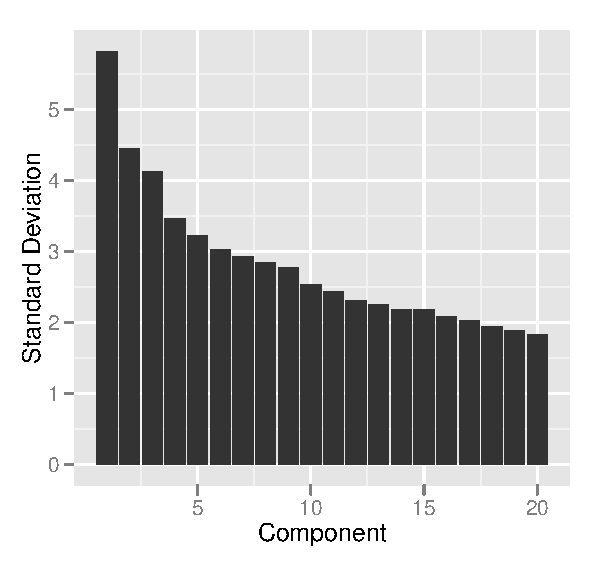
\includegraphics[scale=0.65]{components.pdf}
\caption{Variances of each of the first twenty components obtained from PCA.}
\label{components}
\end{figure}


Let us see how dimension-reduced analysis will compare to previous methods. As usual, we are performing a five-fold validation procedure. We run PCA on the training set to extract four principal components, and their mixing coefficients for each observation. We then fit the response variable to these four dimensions using several regression algorithms. Finally, we calculate the mixing coefficients using the same principal components, but in the testing set, and use them to predict C1. 


\begin{center}
\begin{table*}[ht]
\begin{tabular}{l l l l}
\hline \hline
Component 1 & Component 2 &Component 3&Component 4\\ \hline 
first drank alcohol regularly &		grade point average		&money from a job or other work&money from a job or other work\\
first used marijuana  &		drink too much estimate	&age					&	abstainers\\
first smoked a cigar&		abstainers estimate		&time spent working for wages	&time spent working for wages\\
high school-drink per time&watching tv			&abstainers estimate		&drink too much estimate\\
max drinks male&		max drinks male		&drink too much estimate		&money from other resources\\
\hline
\end{tabular}
\caption{Top five terms in each component.}
\label{components}
\end{table*}
\end{center}

Predictive error using three different regression algorithms after PCA are plotted in Fig. \ref{linear_plus_pca}. Using the best regression algorithm on data with three and four feature classes gave a slightly higher (\textasciitilde 0.6) error. However, it did so by only using four numbers instead of two hundred, which is impressive.

%actually gave a lower error after PCA than without PCA! In the end, four principal components were sufficient to encode 200+ variables.
\begin{figure}[t]
\centering
\makebox[\textwidth][c]{
\subfigure[]{
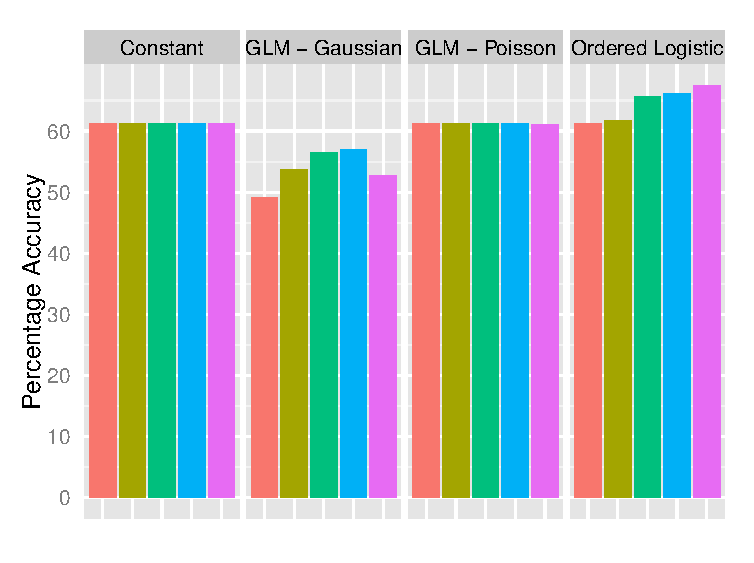
\includegraphics[scale=0.65]{error_percent_pca.pdf}
\label{linear_plus_pca_percent}
}
\subfigure[]{
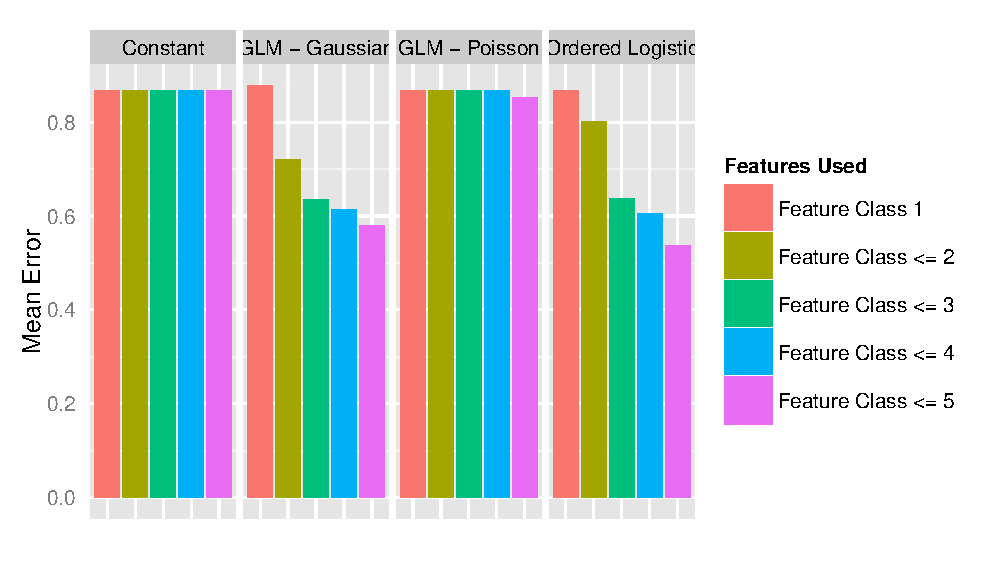
\includegraphics[scale=0.65]{error_pca.pdf}
\label{linear_plus_pca_error}
}
}
\caption{Regression after PCA: Predictive accuracy and mean error of each algorithm using various feature classes.}
\label{linear_plus_pca}
\end{figure}
